\chapter{LUNES}
I lavoro di tesi prevede una simulazione su base realistica del funzionamento della blockchain utilizzata per i Bitcoin al fine di effettuare analisi su possibili attività malevole che sono state fino ad ora solo formulate.

Questa necessità impone l'utilizzo di reti \textit{peer-to-peer}, un notevole numero di nodi, la possibilità di raccogliere dei dati a precisi timestamp e la possibilità di inserire alcuni scenari da applicare alla rete (\textit{forking attack}, \textit{Sybil attack}, \textit{51\%}).\newline\newline
Innanzitutto è fondamentale ricostruire lo stack del protocollo Bitcoin evitando quelle caratteristiche che lo rendono difficoltoso da simulare: mining, dimensione della blockchain, transazioni e decentralizzazione.\newline
Il mining deve essere una caratteristica controllata dall'analista in quanto è un fattore importante nell'analisi dei dati e, in aggiunta, non può rispecchiare tempistiche, dimensioni e difficoltà della rete attuale.\newline
Per quanto riguarda le transazioni e la decentralizzazione è necessario che la simulazione non interagisca con la reale rete di peer di Bitcoin ma che il tutto sia coordinato dal simulatore.\newline
Il primo problema fondamentale da risolvere è la simulazione di reti \textit{peer-2-peer} in quanto per loro natura sono non-strutturare e i collegamenti sono effettuati arbitrariamente e localmente. Un altro problema consiste nel progettare una struttura che utilizzi il protocollo di gossip per simulare l'interazione tra nodi Bitcoin senza però l'obiettivo di creare moneta o decentralizzazione ma rispettando le caratteristiche del protocollo Bitcoin ed in maniera efficiente e scalabile. L'obiettivo infatti è raggiungere una dimensione della rete \textit{p2p} che sia paragonabile con quella reale. La rete di simulazione deve essere sufficientemente grande da garantire che i risultati ottenuti siano spendibili e applicabili alla rete reale: un test eseguito su un numero ristretto di peer potrebbe portare ad analisi non corrette in quanto il fattore di randomizzazione della rete è applicato a meno peer\footnote{Con un campione ristretto esiste un maggior rischio che la rete \textit{p2p} sia completamente connessa e che i fattori come latenza, posizione nella rete possano rendere un attacco molto più (o meno) probabile.}.
\begin{figure}
    \centering
    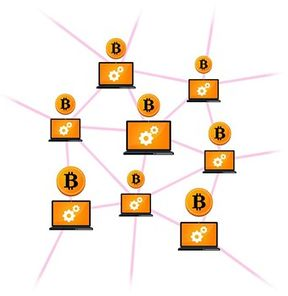
\includegraphics[width=0.5\textwidth]{images/peer2peer_bitcoin.png}
    \source{bitcoinwiki.org}
\end{figure}

\section{Peer-2-Peer}
L'assenza di una struttura nelle reti \textit{p2p} ne facilita la gestione ma al costo non ottimale per la distribuzione dei messaggi: non è possibile prevedere ad esempio gli esatti destinatari di un messaggio senza incorrere un ripetizioni.
In una rete non strutturata i collegamenti tra i nodi sono effettuati arbitrariamente e localmente.
Lo schema di diffusione deve garantire però la copertura della maggior parte della rete con alta probabilità (ad esempio con approcci basati su [\_gossip\_](https://en.wikipedia.org/wiki/Gossip\_protocol)). L'algoritmo viene utilizzato in ambienti come sistemi ad-hoc, multicast, giochi multiplayer online, sistemi distribuiti virtuali, reti di sensori, reti opportunistiche, sistemi di publish-subscribe, query su dati XML, scoperta di risorse, gestione delle risorse in ambienti di cloud computing e sistemi distribuiti, social network, etc.
Ad esempio Amazon S3 utilizza il protocollo gossip per inviare le informazioni sullo stato dei server nel sistema, in Facebook è stato sviluppato \_Cassandra\_ come sistema di storage distribuito utilizzando una strategia gossip (\_Scuttlebutt\_) per la gestione e l'invio dei messaggi di controllo degli stati.
Il simluatore si basa su una architettura distribuita e parallela.

Una rete overlay è una rete costruita sopra un'altra rete utilizzando i nodi di quest'ultima.

The main goal of LUNES is the efficient simulation of complex protocols on top of large scale, unstructured networks. It offers an efficient and easy-to-use tool for the simulation of complex protocols on top of large graphs. In practice, LUNES is able to import the graph topologies generated by other tools (e.g. igraph) and provides the functionalities that are needed for the performance evaluation of simulated protocols. LUNES has been designed to clearly split the fundamental phases: 1) network topology creation; 2) protocol simulation in a specific testbed; 3) traces analysis (i.e. performance evaluation). This modular approach permits the easy integration of external software tools. In practice, such integration is based on very simple template files (such as the graphviz dot language) and provides a good level of extensibility. Under the performance and scalability viewpoint, the most demanding points are the protocol simulation and the traces analysis. The first one is demanded to the ARTÌS middleware and the GAIA/GAIA+ framework, such tools are based on the Parallel And Distribute Simulation (PADS) approach and provide a very good level of scalability. LUNES has been written in such a way to be able to exploit the adaptive re-configuration features provided by GAIA+. The second one, that is the traces analysis, has been excluded from the simulation tasks and some specific software tools have been implemented. Also in this case, the design and implementation of such tools has been done in such a way to exploit all the computational resources provided by parallel (multi-processor or multi-core) architectures.

## Gossip-style protocol

Il protocollo gossip è un tipo di protocollo \_epidemico\_ semplice ma efficace per diffondere informazioni. Il fattore chiave è l'utilizzo della randomizzazione per la propagazione dei dati.
La comunicazione può essere:

* \_push\_ il mittente decide quale nodo riceverà il messaggio
* \_pull\_ i destinatari scelgono come avviare una comunicazione con un altro noto che invierà i dati
* \_push-pull\_ entrambi i noti mittente e destinatario condividono i proprio dati tramite gossip

A secondo che si utilizzi uno schema SIR (\_Susceptible\_ - \_Infective\_ - \_Recovered\_) o SIS (\_Susceptible\_ - \_Infective\_ - \_Susceptible\_) è una pratica comune impiegare un meccanismo di caching dei messaggi; in questo modo lo schema diventa SIRS.

## Protocollo di diffusione

Ogni nodo riceve un messaggio e lo invia a tutti i nodi a cui è collegato, dopo averlo elaborato, se necessario, e quindi è possibile che un nodo riceva più volte lo stesso messaggio (è un grafo) e che generi traffico nella rete; per evitare ciò si introduce un meccanismo di caching per gli identificativi dei messaggi gia processati e si applica un tempo di vita per un messaggio nella rete (TTL). I messaggi sono elaborati tramite tecnica \_push\_ e i peer conoscono solo i propri vicini.

Per identificare un costo nella disseminazione dei messaggi é utile misurare un rapporto di overhead $ρ$ calcolato come il rapport tra i messaggi consegnati e il numbero minimo di messaggi necessari per una copertura totale (in rete con $n$ nodi e $m$ eventi generati questo valore é $Ω(nm)$ (lower bound)).

Il tuning del parametro $TTL$ é un problema molto importante che impatta le performance del protocollo di disseminazione. Quando viene utilizzato un protocollo di flooding solitamente viene utilizzato un $TTL$ uguale al diametro della rete (che si basa peró su un cammino minimo).

Attualmente il $TTL$ é impostato al 130% del massimo diametro del grafo.

### Probabilitá fissa

La probabilitá di gossip $𝛾$ é fissa ed indipendente da ogni altra caratteristica dei nodi connessi e rappresenta la probabilitá che un messaggio sia inviato ad un vicino ed é dato da $𝛾 = 1/<q>$ (dove $q$ è il valore medio del grado di eccedenza (\_excess degree\_: indica il numero medio dei contatti ottenuti seguento un collegamento)). Esiste una elevata probabilitá di copertura in un grafo randomico quando è probabile che ogni nodo trasmetta un messaggio ad almeno uno dei suoi $<k>$ (in media) nodi vicini; non viene peró preso in considerazione il $TTL$.

```
function INITIALIZATION()
    𝛾 <- CHOOSE\_PROBABILITY()

function DISSEMINATE(msg)
    for all nj in N do
        if RANDOM() < 𝛾 then
            SEND(msg, nj)
        end if
    end for
```

### Trasmissione a broadcast probabilistica

I nodi decidono di inoltrare il messaggio in base ad una certa probabilitá β. Se peró il messaggio é stato generato dal nodo locale allora sará inviato a tutti i nodi vicini.

```
function INITIALIZATION()
    β <- PROBABILITY\_BROADCAST()

function DISSEMINATE(msg)
    if (RANDOM() < β OR FIRST\_TRANSMISSION()) then
        for all nj in N do
            SEND(msg, nj)
        end for
    end if
```

### Gossip dipendente dal grado

La probabilitá di gossip dipende dal grado dei nodi: se un nodo \_m\_ ha grado \_i\_ riceverá un messaggio dal proprio vicino con una probabilitá \_𝛾(i)\_. La funzione \_𝛾(i)\_ è espressa in base ad un parametro $α$ e puó essere espressa come $1/(i ^ α)$ o $1/(ln(αi))$.

## LUNES

**Large Unstructured NEtwork Simulator** (\_LUNES\_) é un tool per la simulazione di protocolli complessi su grafi con arbitraria topologia. Permette sia di creare la rete dei nodi sia l'implementazione del protocollo; in aggiunta comprende anche un modulo per l'analisi dei risultati.
Il tool è stato progettato e costruito per lavorare parallelamente e sfruttare tutte le risorse di comunicazione fornite dalle architetture parallele (multi-core, multi-processor) o distribuite (cluster).

Per la creazione della rete LUNES accetta come modello topologie create da altri strumenti, ad esempio, [\_igraph\_](http://igraph.org/python/).

La raccolta dei dati deve essere eseguita tramite diverse esecuzioni per ottenere dei risultati statisticamente accettabili.

La simulazione di LUNES é demandata al middleware [\_ARTÌS\_](http://www.informatica.unibo.it/it/ricerca/technical-report/2005/UBLCS-2005-01) (\_Advanced RTI System\_) ed al framework [\_GAIA\_](https://cris.unibo.it/handle/11585/614534) (\_Generic Adaptive Interaction Architecture\_).

LUNES, infatti, utilizza delle API ad alto livello fornite da GAIA.

LUNES permette un approccio time-stepped per la simulazione: simplifica il deploy su architetture parallele e distribuite e permette di implementare delle tecniche di load balancing per \_ARTÌS\_ e \_GAIA\_.

L'approccio basato su algoritmi di gossip con migliori performance, in termini di copertura, è quello basato sul grado; nel dettaglio DDF2 è migliore di DDF1.

## ARTÌS: Advanced RTI System

ARTÌS é un middleware adattivo fortemente basato sul riutilizzo delle componenti; orientto alla simulazione parallela e distribuita. In quanto i runtime possono risultato poco trasparenti all'utente finale durante l'esecuzione é stato previsto un meccanismo di real-time introspection attraverso il quale gran parte delle informazioni interne sono rese disponibile tramite publish/subscribe.

La simulazione é time-stepped in quanto il tempo viene suddiviso in step sequenziali di una certa durata: l'avanzare degli step di simulazione non permette che il vincolo di causalita sia mai violato.

La comunicazione avviene tramite un insieme di \_Logical Process (LP)\_ che interagiscono tramite primitive di comunicazione: ogni thread é dedicato alla gestione della comunicazione su un singolo canale di input o output.

Le API per il \_Simulation Manager (SIMA)\_ permettono l'inizializzazione e terminazione della simulazione e gestire le barriere di sicronizzazione:

* $void SIMA Initialize(porta, lps, channel.txt)$: indica al SIMA quanti LP sono presenti e su che porta avveranno le comunicazioni e da quale file leggere le configurazioni dei canali di comunicazione.
  * ```
    # DEFINIZIONE DEI CANALI:
    :MILANO 0
    :BOLOGNA 1
    :ROMA 2
    #DEFINIZIONE DEI LOOKAHEAD
    GLOBAL LA=0 # Look−Ahead Globale Disabilitato
    MILANO: BOLOGNA 5 ROMA 7
    ROMA: MILANO 7 BOLOGNA 3
    BOLOGNA: MILANO 5 ROMA 3
    ```
* $void SIMA Finalize()$: chiude i socket tra SIMA e LP e le risorse allocate in fase di inizializzazione sono rilasciate.
* $void SIMA Barrier()$: istituisce un punto di sicronizzazione.

## GAIA: Generic Adaptive Interaction Architecture

GAIA é un framework per ottimizzare l'esecuzione della simulazione riallocando le entitá, questo riduca i tempi di esecuzione e l'overhead generato dalle comunicazioni sviluppato partendo da ARTÌS.

Una serie di euristiche valutano il pattern di comunicazione ed eventualmente schedulano una riallocazione delle entitá.

Il framework supporta il paradigma a multi agenti (MAS: \_multi-agent system\_) e la possibilitá di eseguire su cluster eterogenei.

## Implementazione LUNES

In $MODELS/LUNES$ c'é sorgente di LUNES con script per la configurazione ed esecuzione del simulatore.

La compilazione ($make$) é necessaria per la creazione degli eseguibili utilizzati per la creazione della rete ($graphgen$), degli agenti ($mig-agents$) e degli eseguibili per i test di coverage.

```java
int     GAIA\_Initialize (int max\_objs\_count, int nlp, String RandFile, String cname, String sima\_host\_name, int sima\_port);
void    GAIA\_Finalize ( );
void    GAIA\_SetFstID (int first\_id);
void    GAIA\_SetHistory (int new\_size);
void    GAIA\_SetMF (int migr\_factor);
void    GAIA\_SetMigration (int state);
void    GAIA\_SetLoadBalancing (int state);
double  GAIA\_GetStep ( );
int     GAIA\_Register (int migrable);
double  GAIA\_TimeAdvance ();
void    GAIA\_Migrate (int id, String data, int size);
void    GAIA\_ByteMigrate (int id, byte[] data, int size);
void    GAIA\_Send (int obj\_src, int obj\_dest, double Ts, String Msg, int Size);
void    GAIA\_ByteSend (int obj\_src, int obj\_dest, double Ts, byte[] Msg, int Size);
void    GAIA\_Broadcast (int obj\_src, double Ts, String Msg, int Size);
void    GAIA\_ByteBroadcast (int obj\_src, double Ts, byte[] Msg, int Size);
String  GAIA\_Receive (int maxlen);
byte[]  GAIA\_ByteReceive (int maxlen);
void    GAIA\_GetStatistics (int local, int remote, int migrations)
```

<http://pads.cs.unibo.it/doku.php?id=pads:gaia-apis>

### $graphgen$

$graphgen$ utilizza la libreria $igraph$ per la creazione di un oggetto C che rappresenta il grapo con i relativi nodi e vertici. La routine attualmente utilizza un modalitá randomica per la creazione del grafo: \_Erdos-Renyi\_.

### Example: Wireless

L'esempio simula un insieme di Mobile Host che si muovono attorno secondo il modello di movimento RWP (Random Way Point) in uno spazio toroidale 2D.

L'interazione tra i vari host avviene per prossiimità.

L'eseguibile prende in ingresso il numero degli LP da utilizzare e degli host da simulare.

I vari host si muovono in base a delle coordinate randomiche nello spazio 2D e una volta raggiunti il punto stabilito inviano un messaggio in broadcast ($GAIA\_Broadcast$) oppure può essere configurato per comunicare con i vicini.

Come in tutte le simulazioni è necessario richiamare le API di GAIA nel main: $GAIA\_Initialize(max\_num\_simulated\_entities, number\_LPs, seed\_file, LP\_name, hostname\_SIMA, port\_SIMA)$ per inizializzare il simulatore; con $GAIA\_Getstep$ è possibile leggere la dimensione di uno step. Si inizializzano anche gli host per LP con $GAIA\_SetFstID$ e il bilanciamento a OFF con $GAIA\_SetLoadBalancing$.

Il core del programma è un loop in cui tramite $GAIA\_Receive$ si legge un messaggio alla volta (conoscendo $from$ e $to$), in base al contenuto del messaggio ($Msg$). Un messaggio è rappresentato da una $union$ in cui è possibile utilizare:

```c
union msg {
    char type;
    LinkMsg link;
    PingMsg ping;
    MigrMsg migr;
    StimulusMsg stimulus;
};
```

Nel caso il messaggio sia:

* $STATE\_CHANGE$: ??? (uguale a $A$)
* $NOTIF\_MIGR$: necessaria migrazione di un SMH (Simulated Mobile Host)
* $NOTIF\_MIGR\_EXT$: migrazione eseguita
* $REGISTER$: registrazione di un nuovo SMH gestita da un altro LP
* $EXEC\_MIGR$: l'LP locale è l'incaricato della migrazione e quindi aggiungere alla lista degli host uno in più
* $EOS$ (\_End Of Step\_): step concluso, se non è la fine della simulazione aggiorna la posizione degli host e ricrea un nuovo step ed esegui la migrazione. In aggiunta salva/stampa le statistiche.
* $UNSET$:  simula cambi di posizione, messaggi di ping e device accessi o spenti

Infine è necessario finalizzare il simulatore $GAIA\_Finalize$ e liberare la memoria.

\section{NS-3}
NS-3 è un simulatore di rete ad eventi discreti, destinato principalmente alla ricerca e all'utilizzo educativo. Il progetto è impegnato nella costruzione di un solido nucleo di simulazione ben documentato, di facile debug e che soddisfa le esigenze dell'intero flusso di lavoro, dalla configurazione alla raccolta dati. Il design del simulatore è studiato per supportare simulazioni su reti IP ma una buona estendibilità lo rende in grado di lavorare anche con altri protocolli (ndnSIM ne è un esempio).Esso dispone di uno scheduler Realtime ingrado di gestire in maniera dinamica gli eventi istanziati dai nodi che compongono la topologia di rete.
La struttura è simile a quella di una libreria che può essere collegata staticamente o dinamicamente a un programma principale C++ che definisce la topologia e lancia la simulazione. Tutte le API sono esportate anche in Python.
Le fondamenta di ns-3 sono racchiuse nei moduli Core e Network dove vengono implementate genericamente le caratteristiche fondamentali di un simulatore di rete (non solo reti IP);
Core descrive gli aspetti fondamentali di qualunque protocollo mentre Network definisce la struttura dei pacchetti. Proprio sopra questi due livelli vedremo come verrà integrato ndnSIM.
Questa solida base permette ad ns-3 di andare a sviluppare nei livelli superiori aspetti di maggiore dettaglio come applicazioni, dispositivi di rete, modelli di movimento e modelli di propagazione. Infine, ns-3 sviluppa una serie di convenienti API wrapper chiamati Helper che facilitano notevolmente le chiamate a primitive di basso livello.

% NeoTex: mainfile=main.tex:
